\subsection{Fatos estilizados da economia norte-americana}\label{FatosEUA}

%Desse modo, a literatura do supermultiplicador é um contraponto ao \textit{trade-off} apontado por \textcite{solow_importance_1995} uma vez que são os gastos autônomos que lideram o crescimento no longo prazo.

%TODO Rever início da seção.

INTRODUÇÃO

A participação do investimento das firmas em relação tanto ao PIB quanto aos trabalhos que o analisam é bastante superior a do investimento das famílias. Tal pequenez, no entanto, não implica em menor relevância para a dinâmica macroeconômica nem --- ao contrário do que indicaria a intuição --- em menor volatilidade.
Dito isso, o objetivo desta seção é evidenciar que a pouca atenção dada ao investimento residencial não é compatível com seu grau de importância para a economia norte-americana e que esta relevância não se restringe à crise imobiliária recente.

PEQUENA PARTICIPAÇÃO NO PIB

\begin{figure}[htb]
	\centering
	\caption{Participação dos gastos autônomos no PIB}
	\label{FigVolatilidade}
	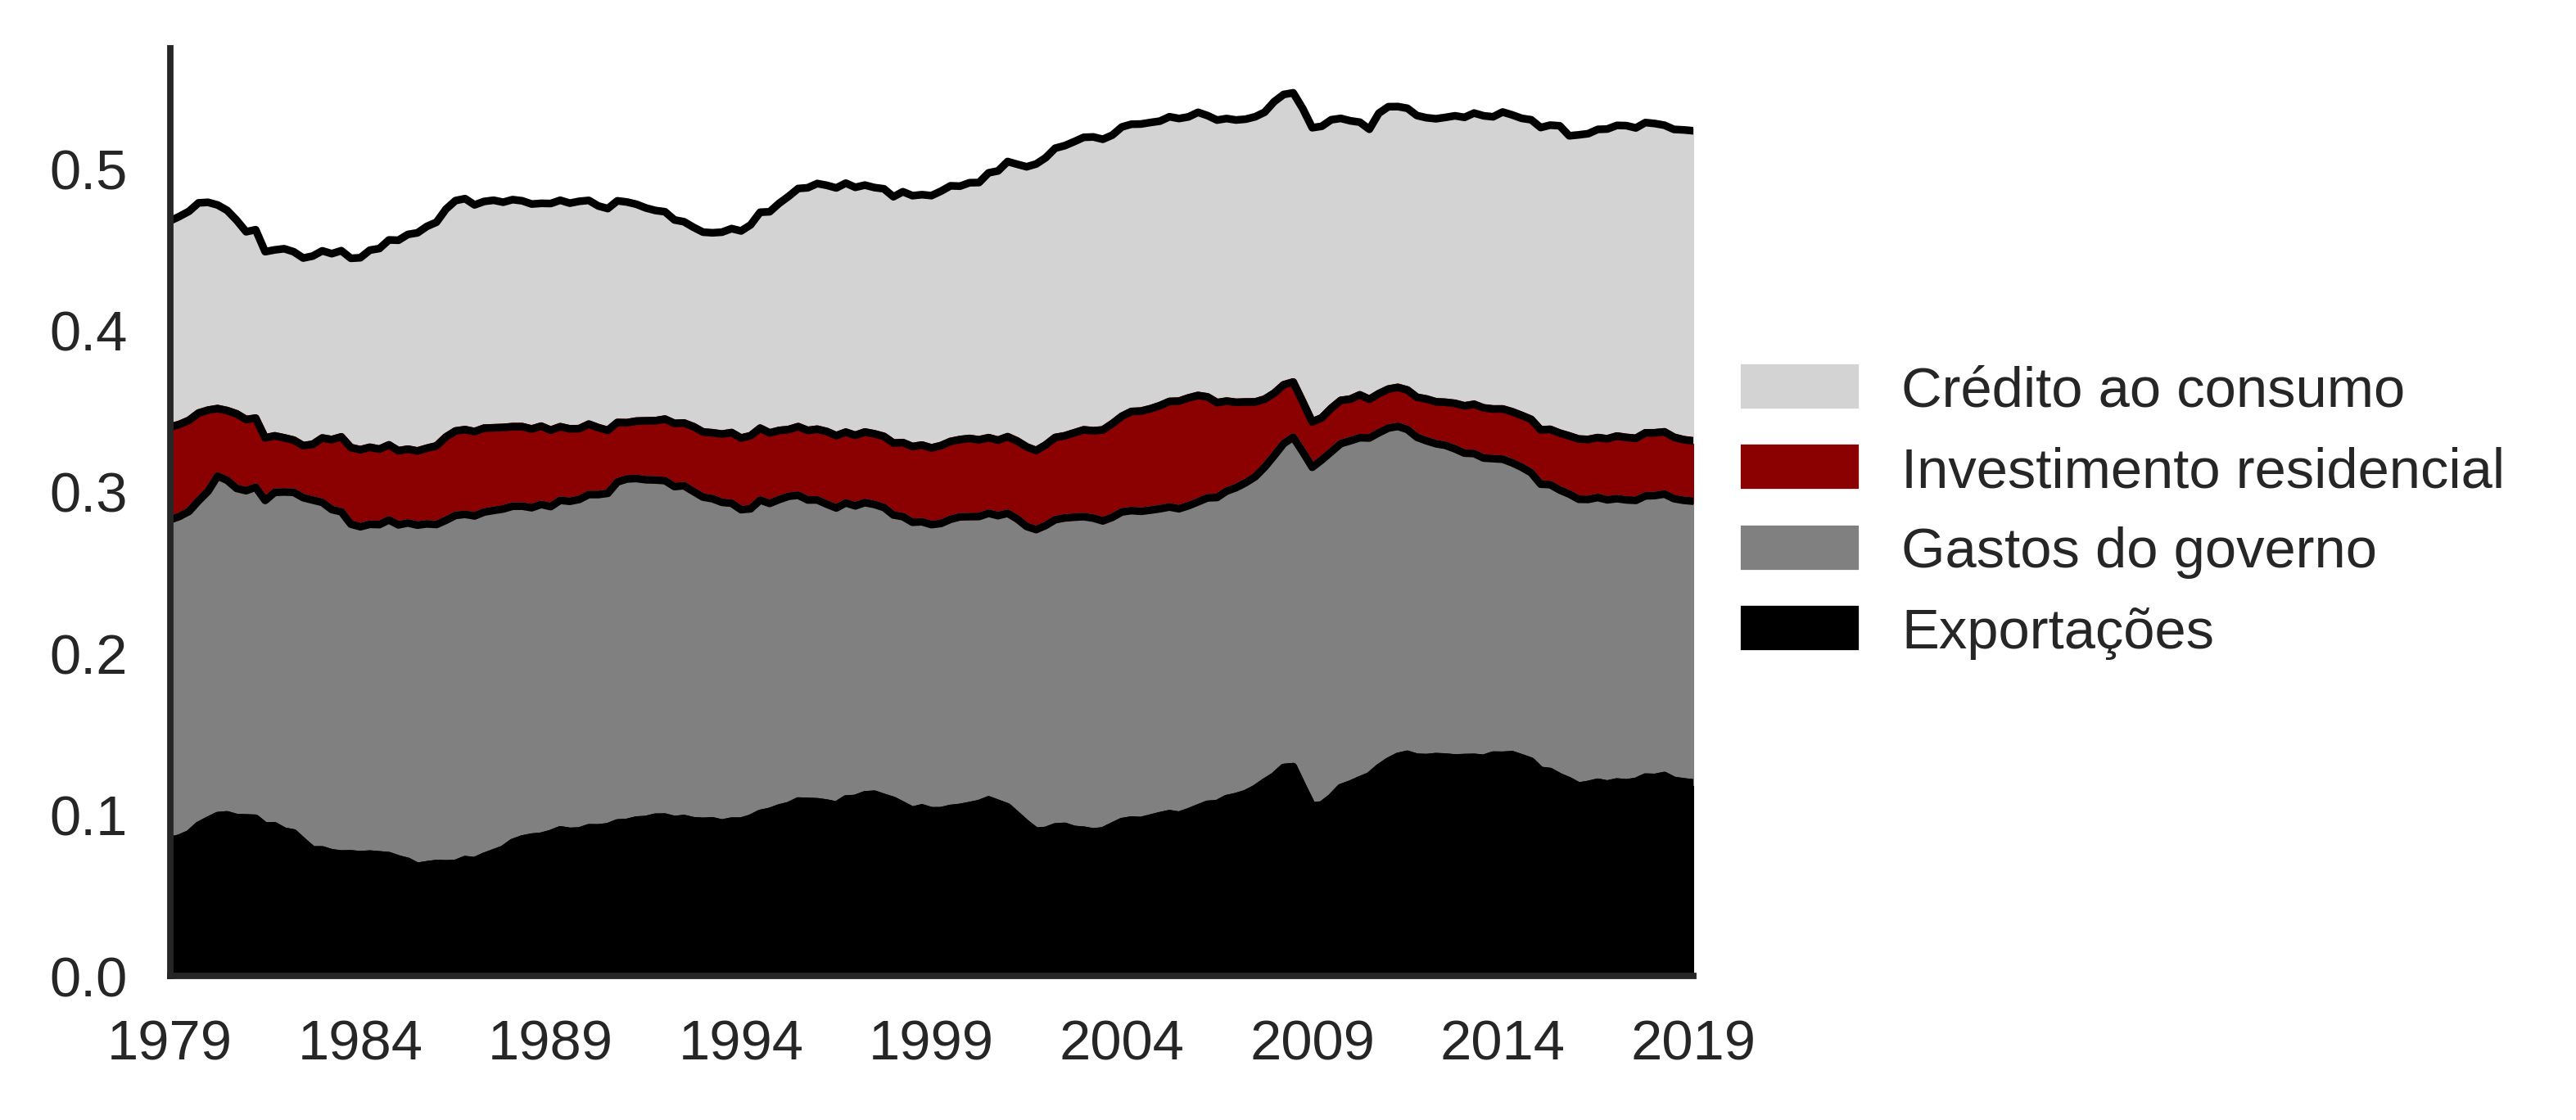
\includegraphics[width=\textwidth]{../../Dados/Fatos_Estilizados/figs/Gastos_autonomos.png}
	\caption*{\textbf{Fonte:} U.S. Bureau of Economic Analisys, elaboração própria}
\end{figure}


\begin{figure}[htb]
	\centering
	\caption{Volatilidade de taxas de crescimento selecionadas (pré e pós-crise \textit{subprime})}
	\label{FigVolatilidade}
	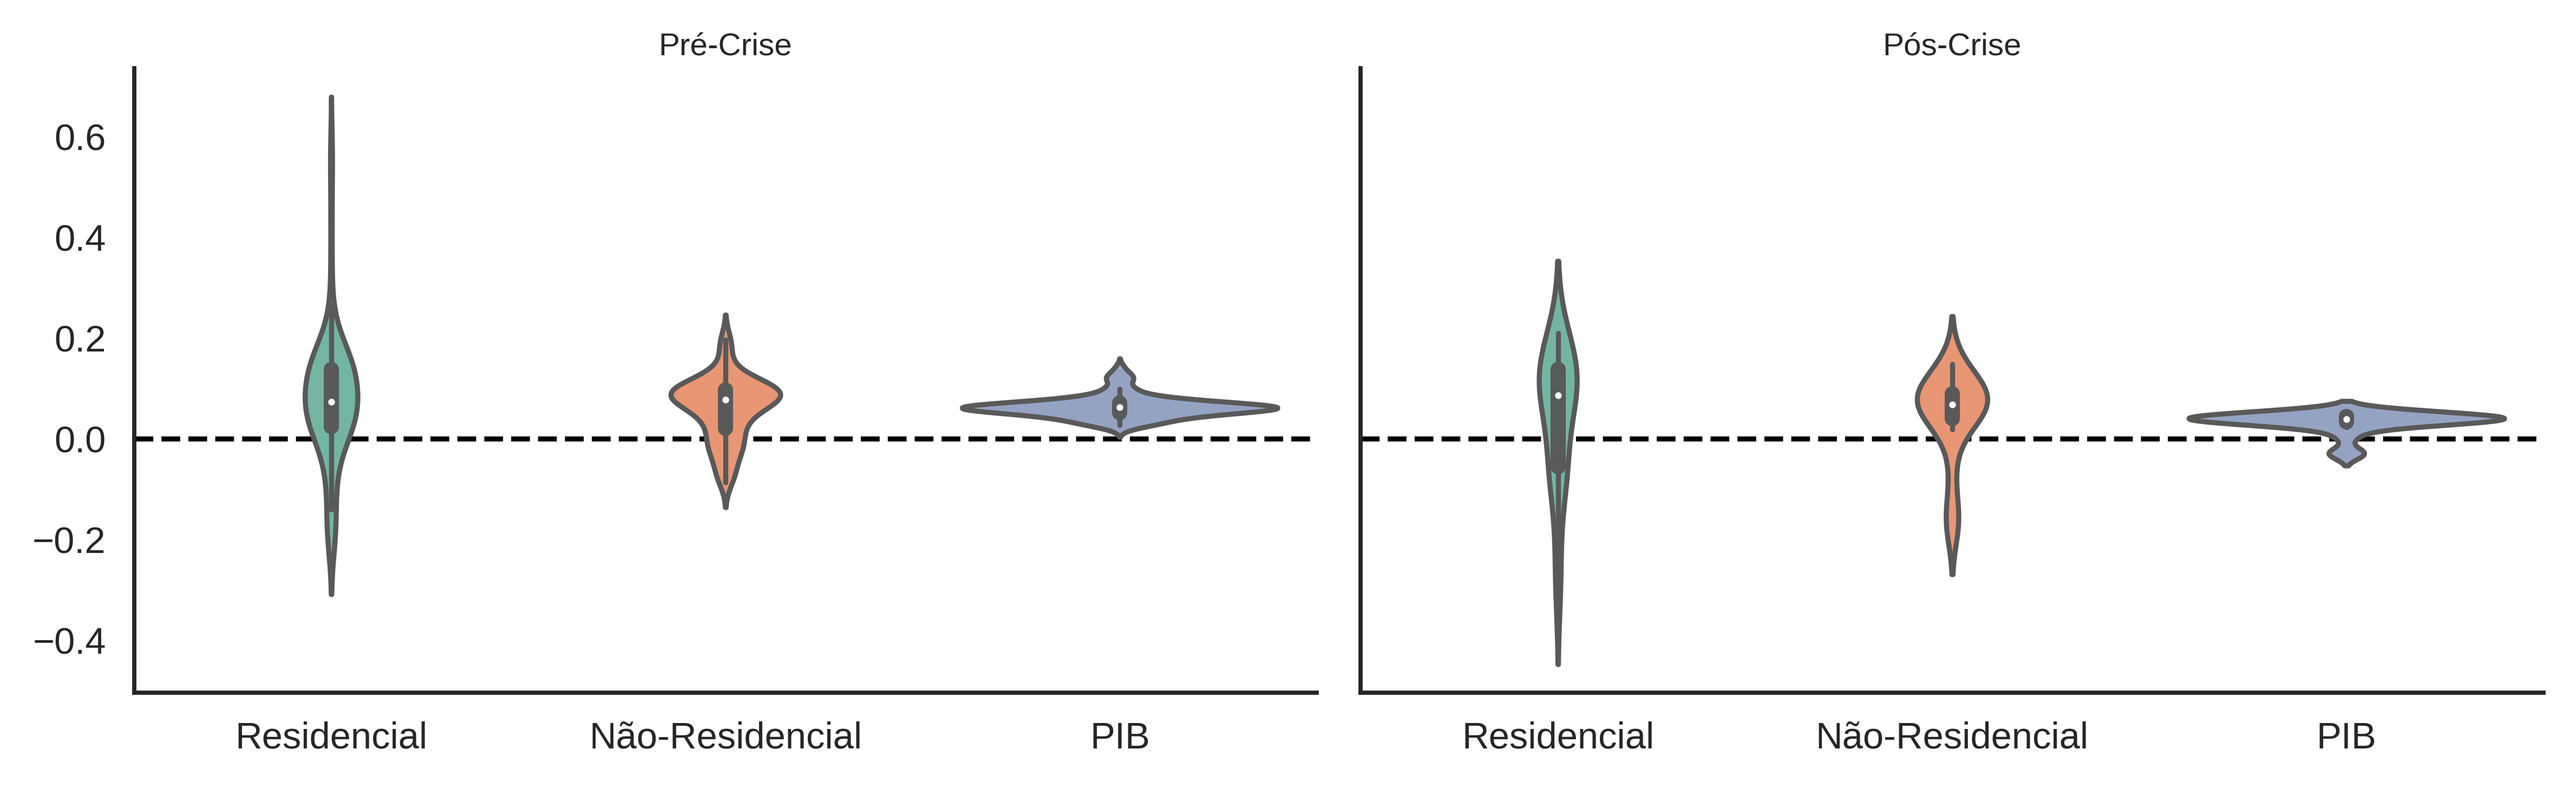
\includegraphics[width=\textwidth]{../../Dados/Fatos_Estilizados/figs/Volatilidade.png}
	\caption*{\textbf{Fonte:} U.S. Bureau of Economic Analisys, elaboração própria}
\end{figure}

ELEVADA VOLATILIDADE

Neste ponto, cabe mencionar o ineditismo de \textcite{green_follow_1997} e \textcite{leamer_housing_2007} --- e revisitado em \textcite{leamer_housing_2015} e por \textcite{fiebiger_trend_2017} --- ao lançar luz sobre a importância do investimento residencial na determinação dos ciclos econômicos antes mesmo da crise dos \textit{subprimes}. 
Ao avaliar o caso norte-americano, \textcite{green_follow_1997} conclui que o investimento residencial possui uma capacidade preditiva maior que o investimento das firmas, mas que isso não implica no estabelecimento de uma relação causal. Na tentativa de compreender tais resultados, afirma:

\begin{citacao}
	
	[P]erhaps residential investiment, like stock prices and interest rates, is a good predictor of GDP because it is a series that reflects \textbf{foward looking behavior}. Presumably households will not increase their expenditures on housing unless they expect to prosper in the future. Building a house is a natural mechanism for doing this. Thus, the series can do a good job of predicting GDP without necessarily causing GDP.
	\cite[p.~267, grifos adicionados]{green_follow_1997}
\end{citacao}
Apesar de dar atenção para um gasto não criador de capacidade, o argumento de \textcite{green_follow_1997} se difere das conclusões do supermultiplicador uma vez que não são estes gastos que lideram o crescimento.
\textcite{leamer_housing_2007}, por sua vez, avança em direção a relação de causalidade entre este gasto e o PIB. Grosso modo, afirma que a construção de novos imóveis implica em maior consumo de bens duráveis e, portanto, trata-se de um ciclo decorrente do \textit{volume} e não do preço dos imóveis. 

Uma forma de visualizar a importância do investimento residencial para o ciclo econômico na economia estadunidense é por meio do gráfico \ref{Investo_Resid} em que cada um dos painéis apresenta um ciclo iniciado no primeiro trimestre de crescimento positivo após a recessão\footnote{
	Raciocínio semelhante pode ser encontrado em \textcite{fiebiger_semi-autonomous_2018} em que, diferentemente do presente trabalho, não é incluído consumo financiado por crédito.}. 
No eixo vertical, observa-se a participação desse gasto no PIB, enquanto no eixo horizontal, o grau de utilização da capacidade como uma \textit{proxy} para o ciclo econômico. Exceto para o período 1991-2001, a recuperação (aumento da utilização da capacidade) é caracterizada por uma taxa de crescimento do investimento residencial maior que o crescimento da economia, resultando em maior participação desse gasto no PIB. Considerando que as firmas seguem o princípio do ajuste do estoque de capital, ampliam a taxa de acumulação de modo a ajustar o grau de utilização para o grau normal. O aumento da taxa de crescimento do investimento das firmas e de outros gastos reduz a participação do investimento residencial no PIB. A maturação do investimento das firmas, por sua vez, redunda em menor utilização da capacidade produtiva\footnote{
	Complementarmente, os trabalhos de \textcite{fiebiger_semi-autonomous_2018} e \textcite{fiebiger_trend_2017} também reportam o investimento residencial como determinante do comportamento cíclico e adicionam o consumo financiado por crédito a essa dinâmica. Além disso, apresentam uma similaridade com \textcite{dejuan_hidden_2017} e \textcite{teixeira_crescimento_2015} para os quais a instabilidade econômica está associada à instabilidade (ao menos de alguns) gastos autônomos e não do investimento das firmas, que segue o princípio do ajuste do estoque de capital.}. 


GRÁFICO RELÓGIO

GRÁFICO RELÓGIO DURÁVEIS

\begin{figure}[htb]
	\centering
	\caption{Relação entre taxa de investimento residencial e grau de utilização por recessão}
	\label{FigIh_u}
	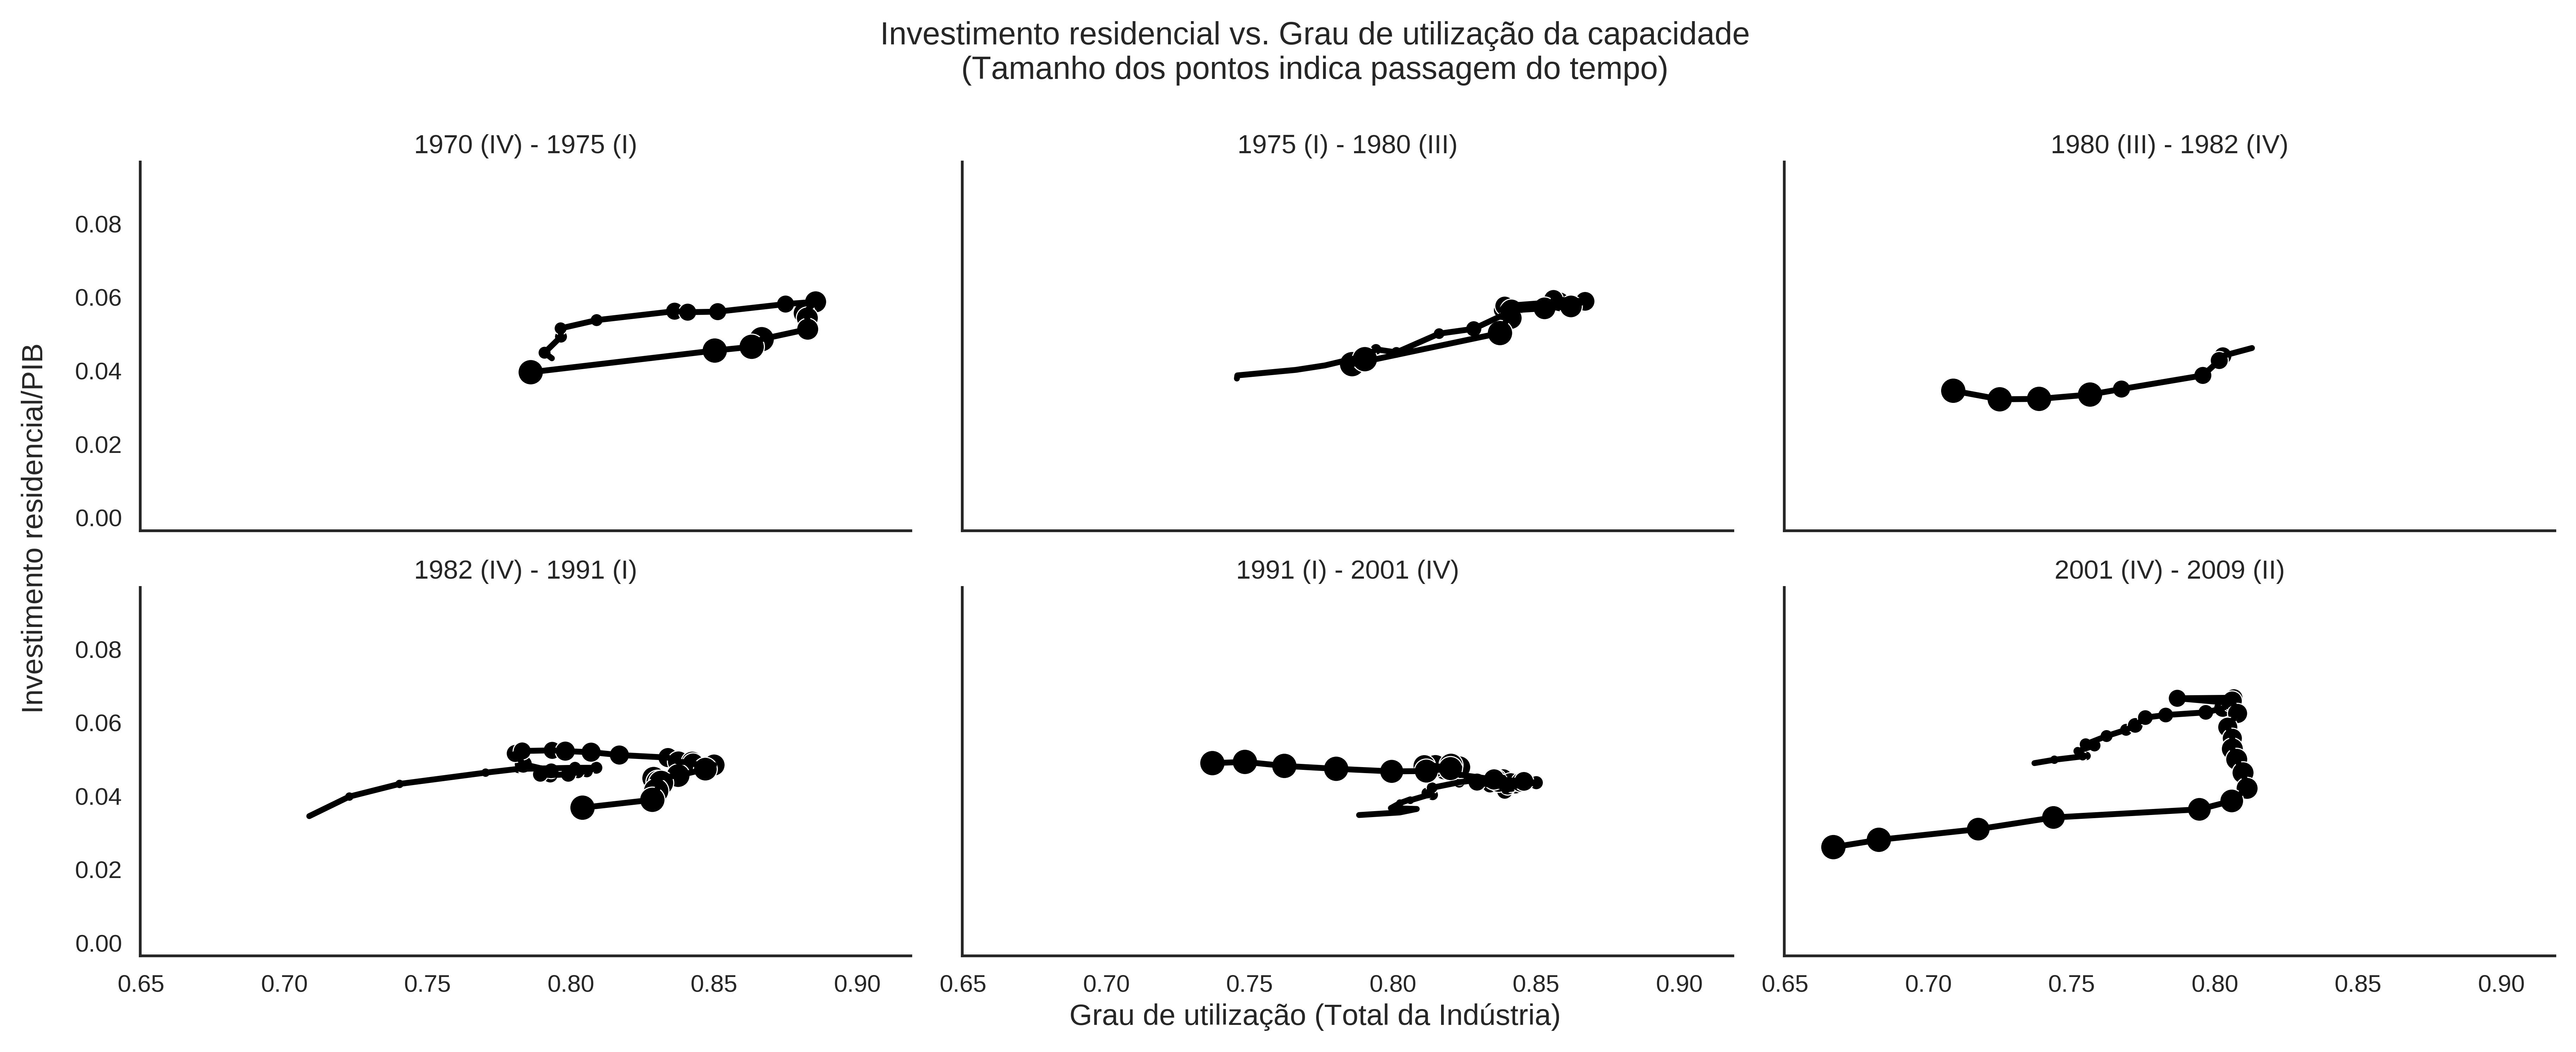
\includegraphics[width=\textwidth]{../../Dados/Fatos_Estilizados/figs/Ciclo_Ih_u.png}
	\caption*{\textbf{Fonte:} Elaboração própria}
\end{figure}

\begin{figure}[htb]
	\centering
	\caption{Relação entre taxa de investimento residencial e grau de utilização por recessão}
	\label{FigInvesto_Duraveis}
	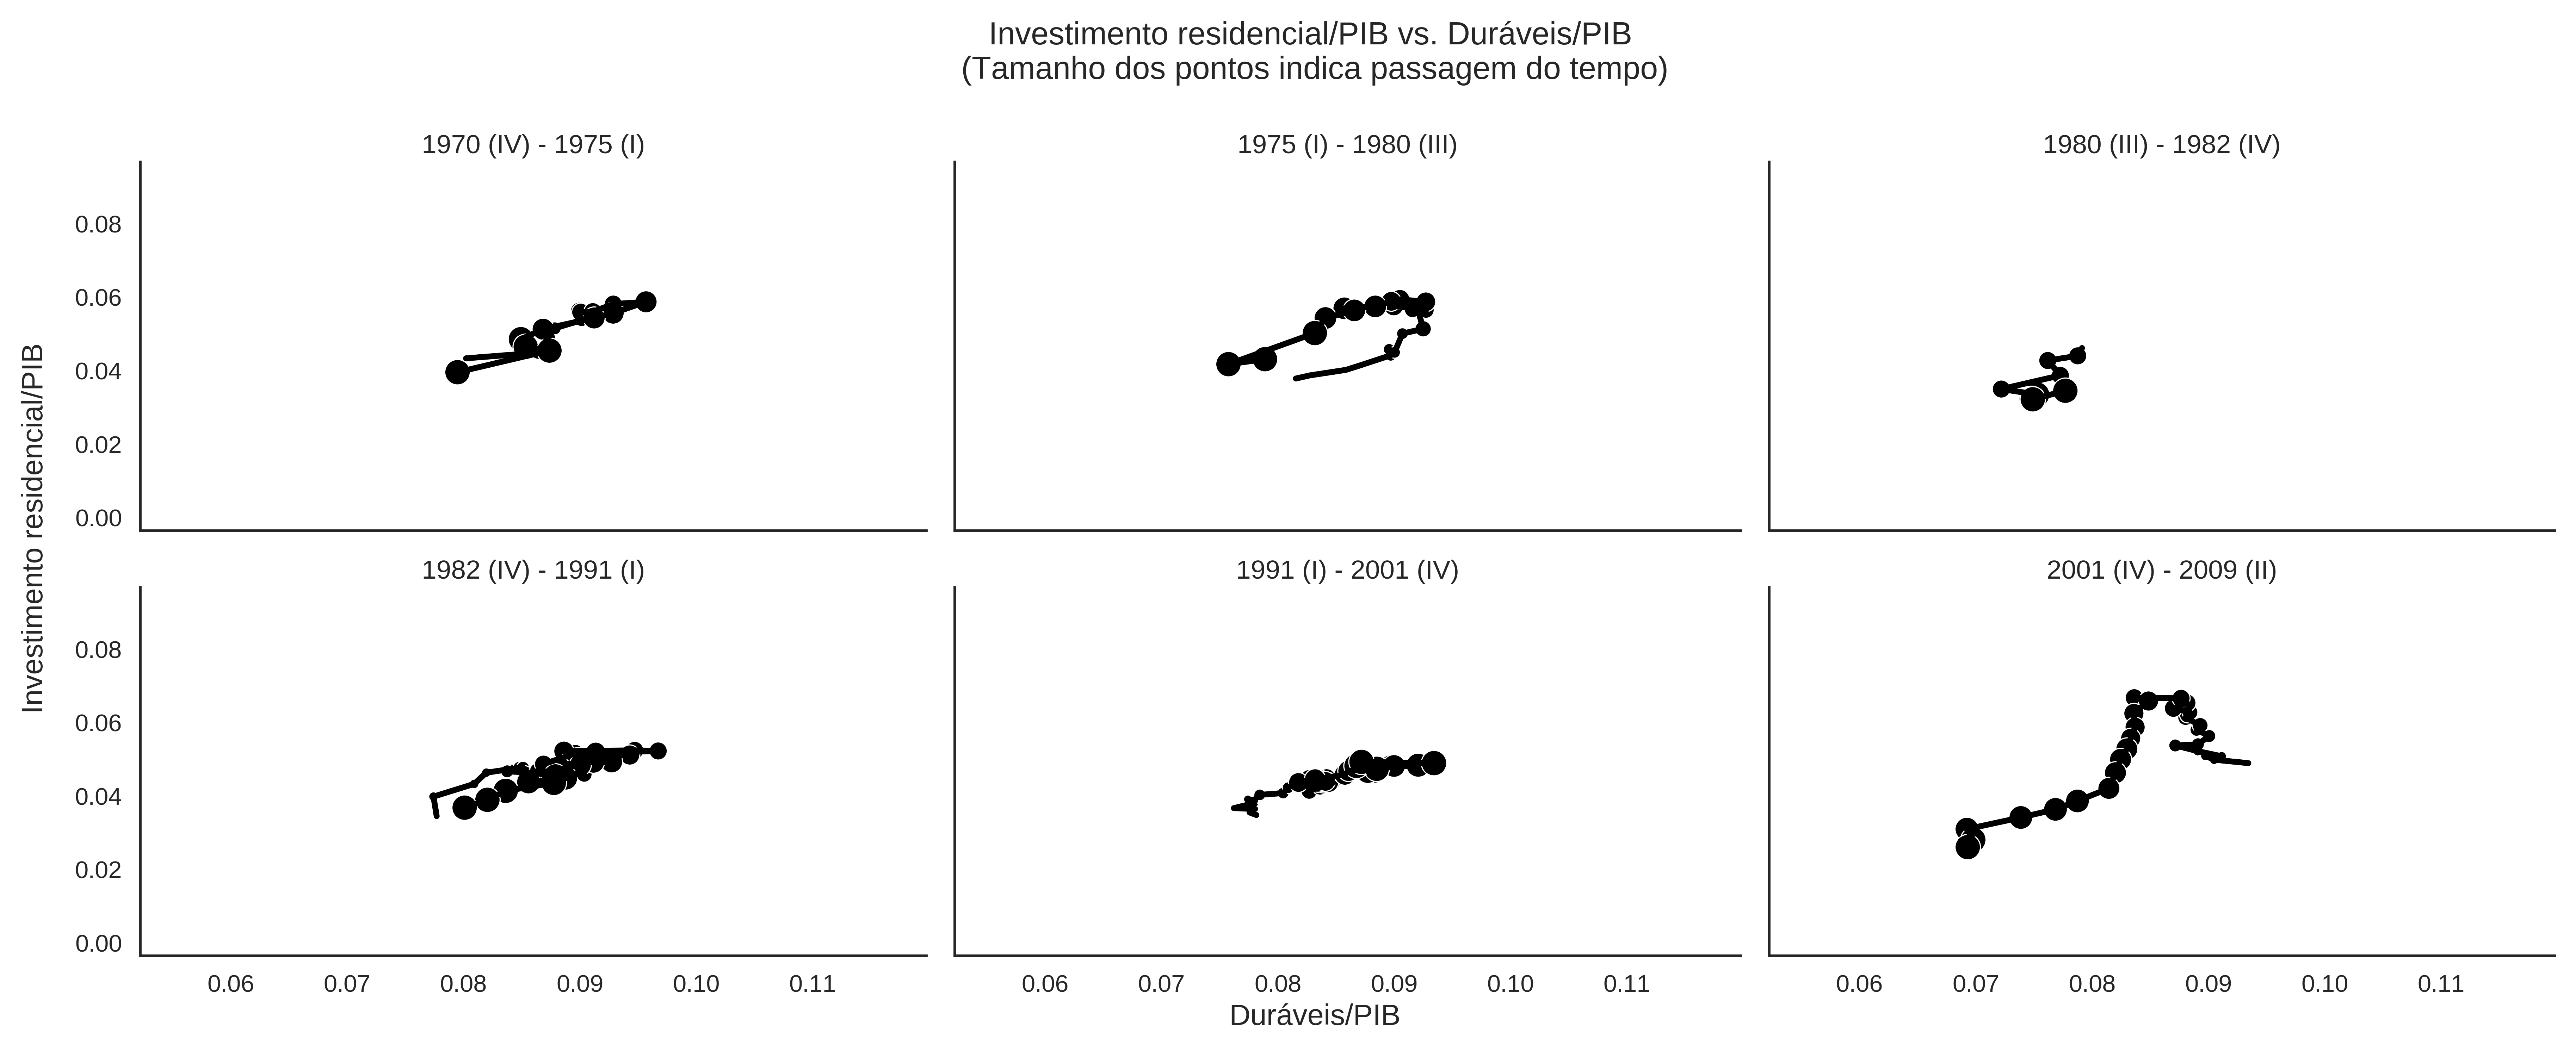
\includegraphics[width=\textwidth]{../../Dados/Fatos_Estilizados/figs/Ciclo_Ih_Duraveis.png}
	\caption*{\textbf{Fonte:} Elaboração própria}
\end{figure}

Desse modo, conclui-se que o investimento residencial ajuda a compreender grande parte das recessões e tal componente de gasto também é significativo para a retomada. Esta dinâmica poder ser visualizada no gráfico \ref{Recuperacao} em que são apresentadas algumas taxas de crescimento\footnote{Neste gráfico, as taxas de crescimento são normalizadas para facilitar a comparatibilidade uma vez que é mantida uma mesma escala.} nos trimestres que antecedem e sucedem as recuperações. Em linhas gerais, observa-se que o investimento residencial possui uma taxa de crescimento (a taxas crescentes) positiva nos trimestres que antecedem a recuperação enquanto o investimento das firmas só apresenta tal comportamento adiante. Portanto, esse gráfico ilustra tanto a capacidade do investimento residencial liderar a retomada quanto a indução do investimento criador de capacidade produtiva.

GRÁFICOS CENTRADOS NORMALIZADOS

\begin{figure}[htb]
	\centering
	\caption{Taxas de crescimento por recessões antes e depois do início da crise (normalizadas pelo desvio-padrão)}
	\label{FigCriseNorm}
	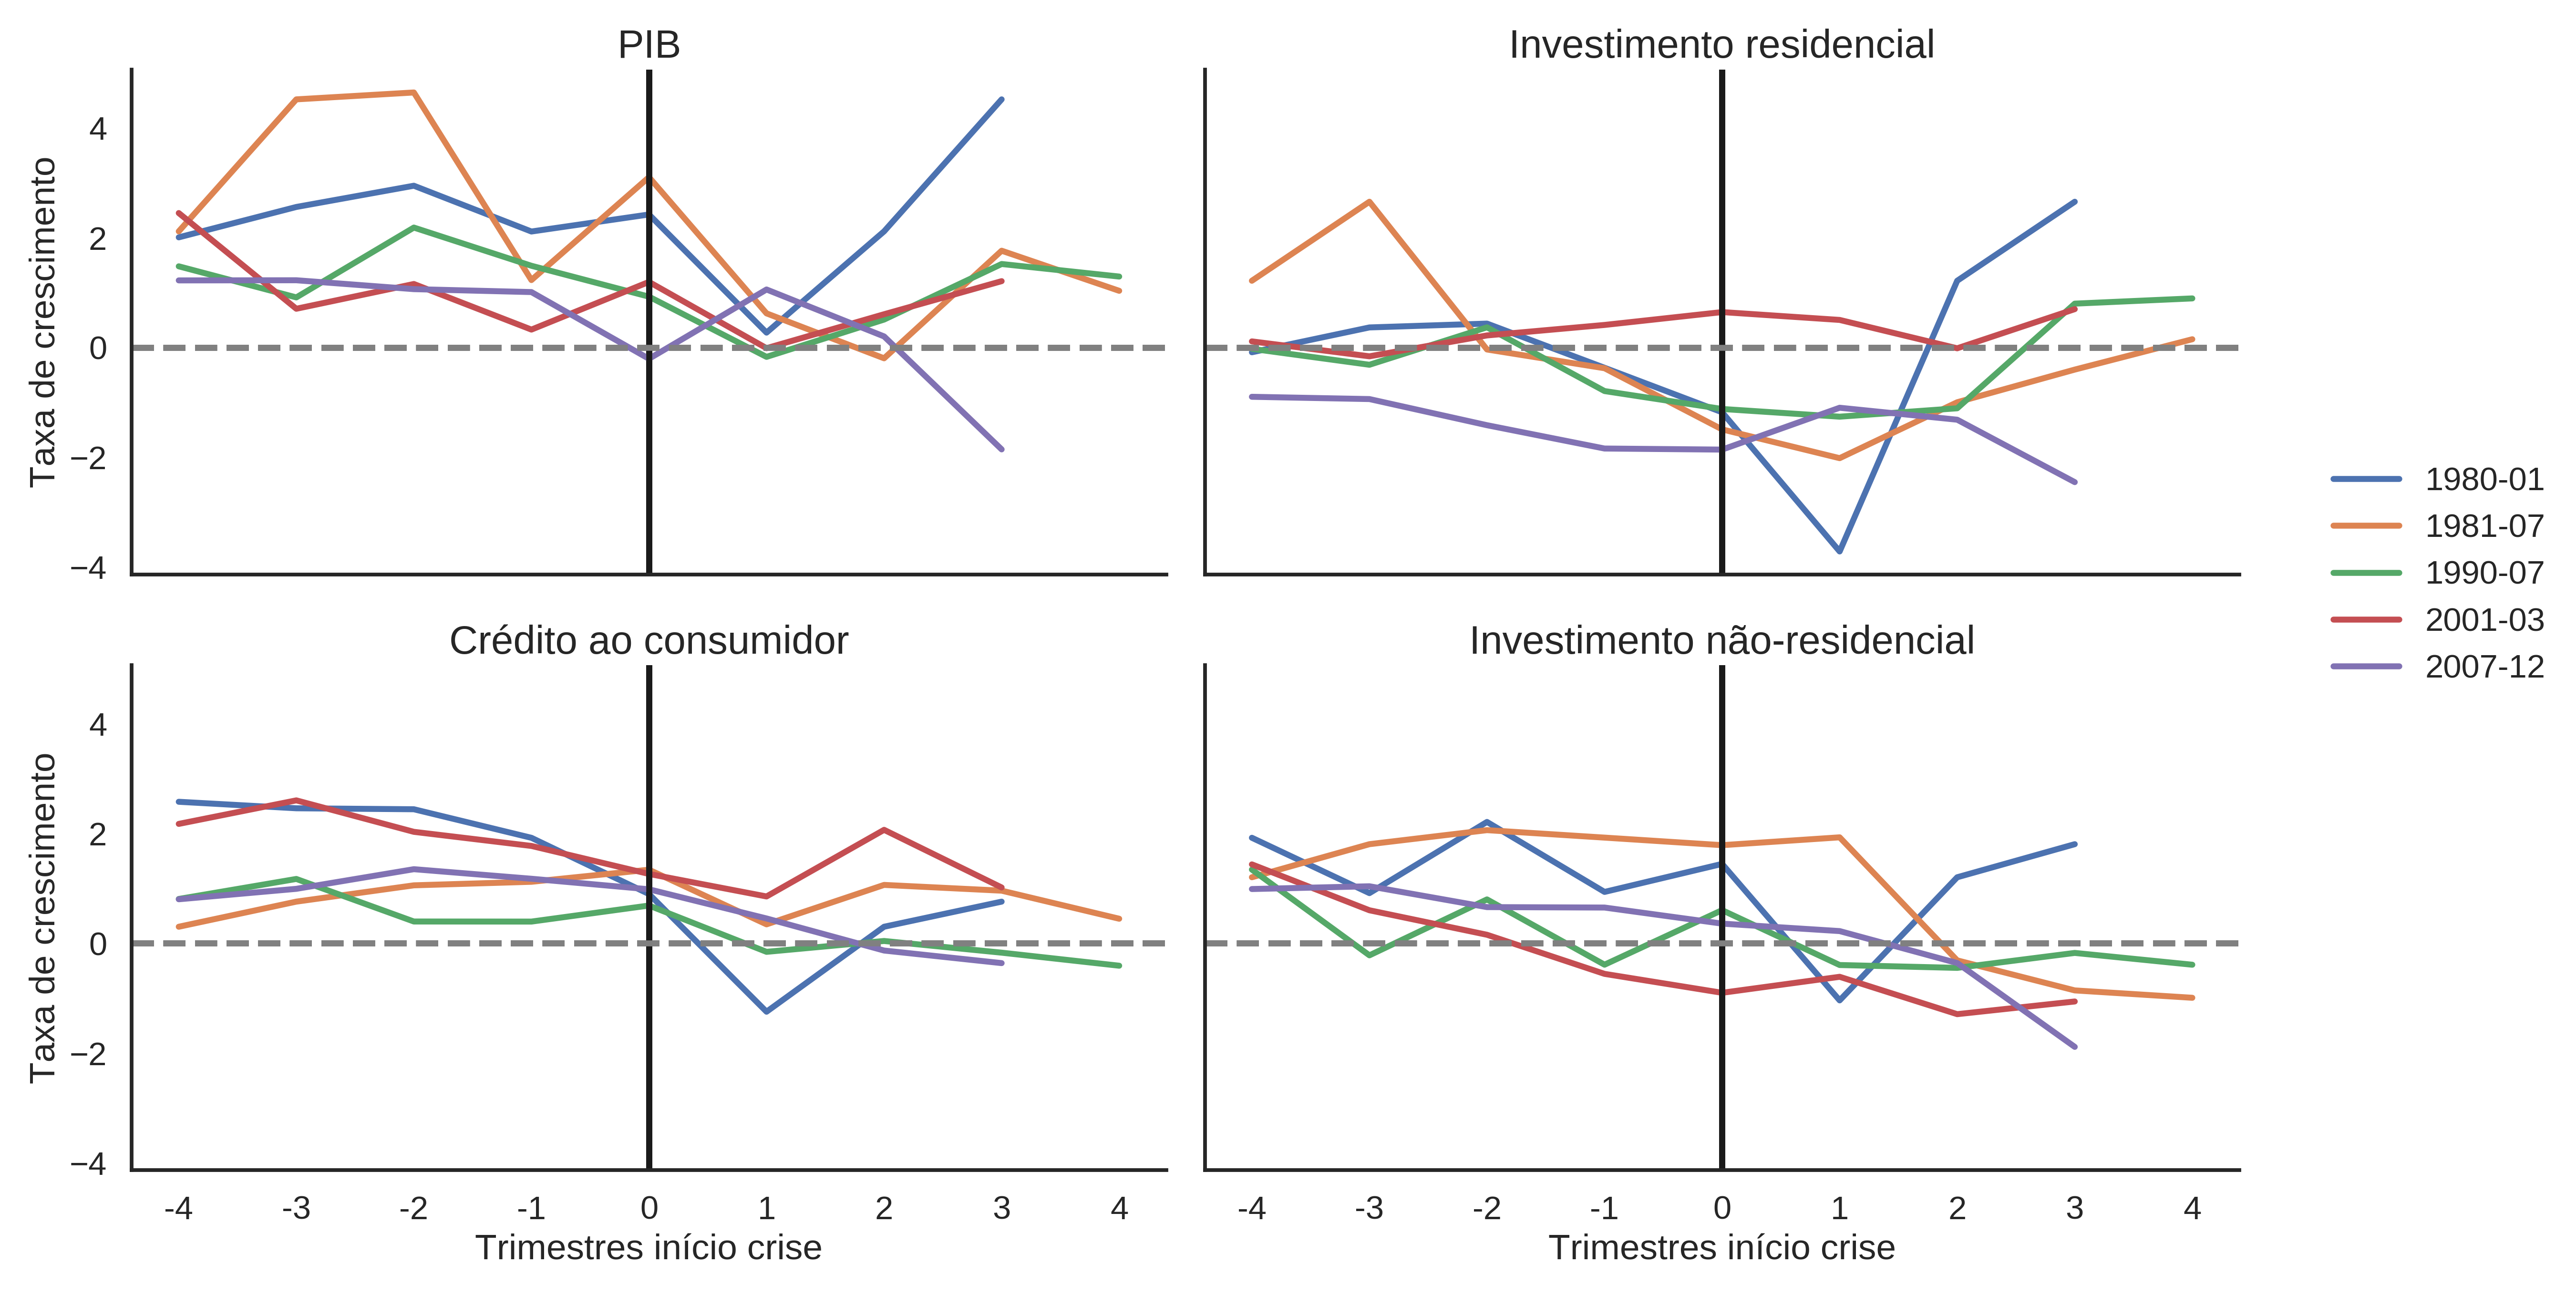
\includegraphics[width=\textwidth]{../../Dados/Fatos_Estilizados/figs/Centrado_Inicio_Norm.png}
	\caption*{\textbf{Fonte:} Elaboração própria}
\end{figure}

\begin{figure}[htb]
	\centering
	\caption{Taxas de crescimento por recessões antes e depois do início da recuperação (normalizadas pelo desvio-padrão)}
	\label{FigRecuperacaoNorm}
	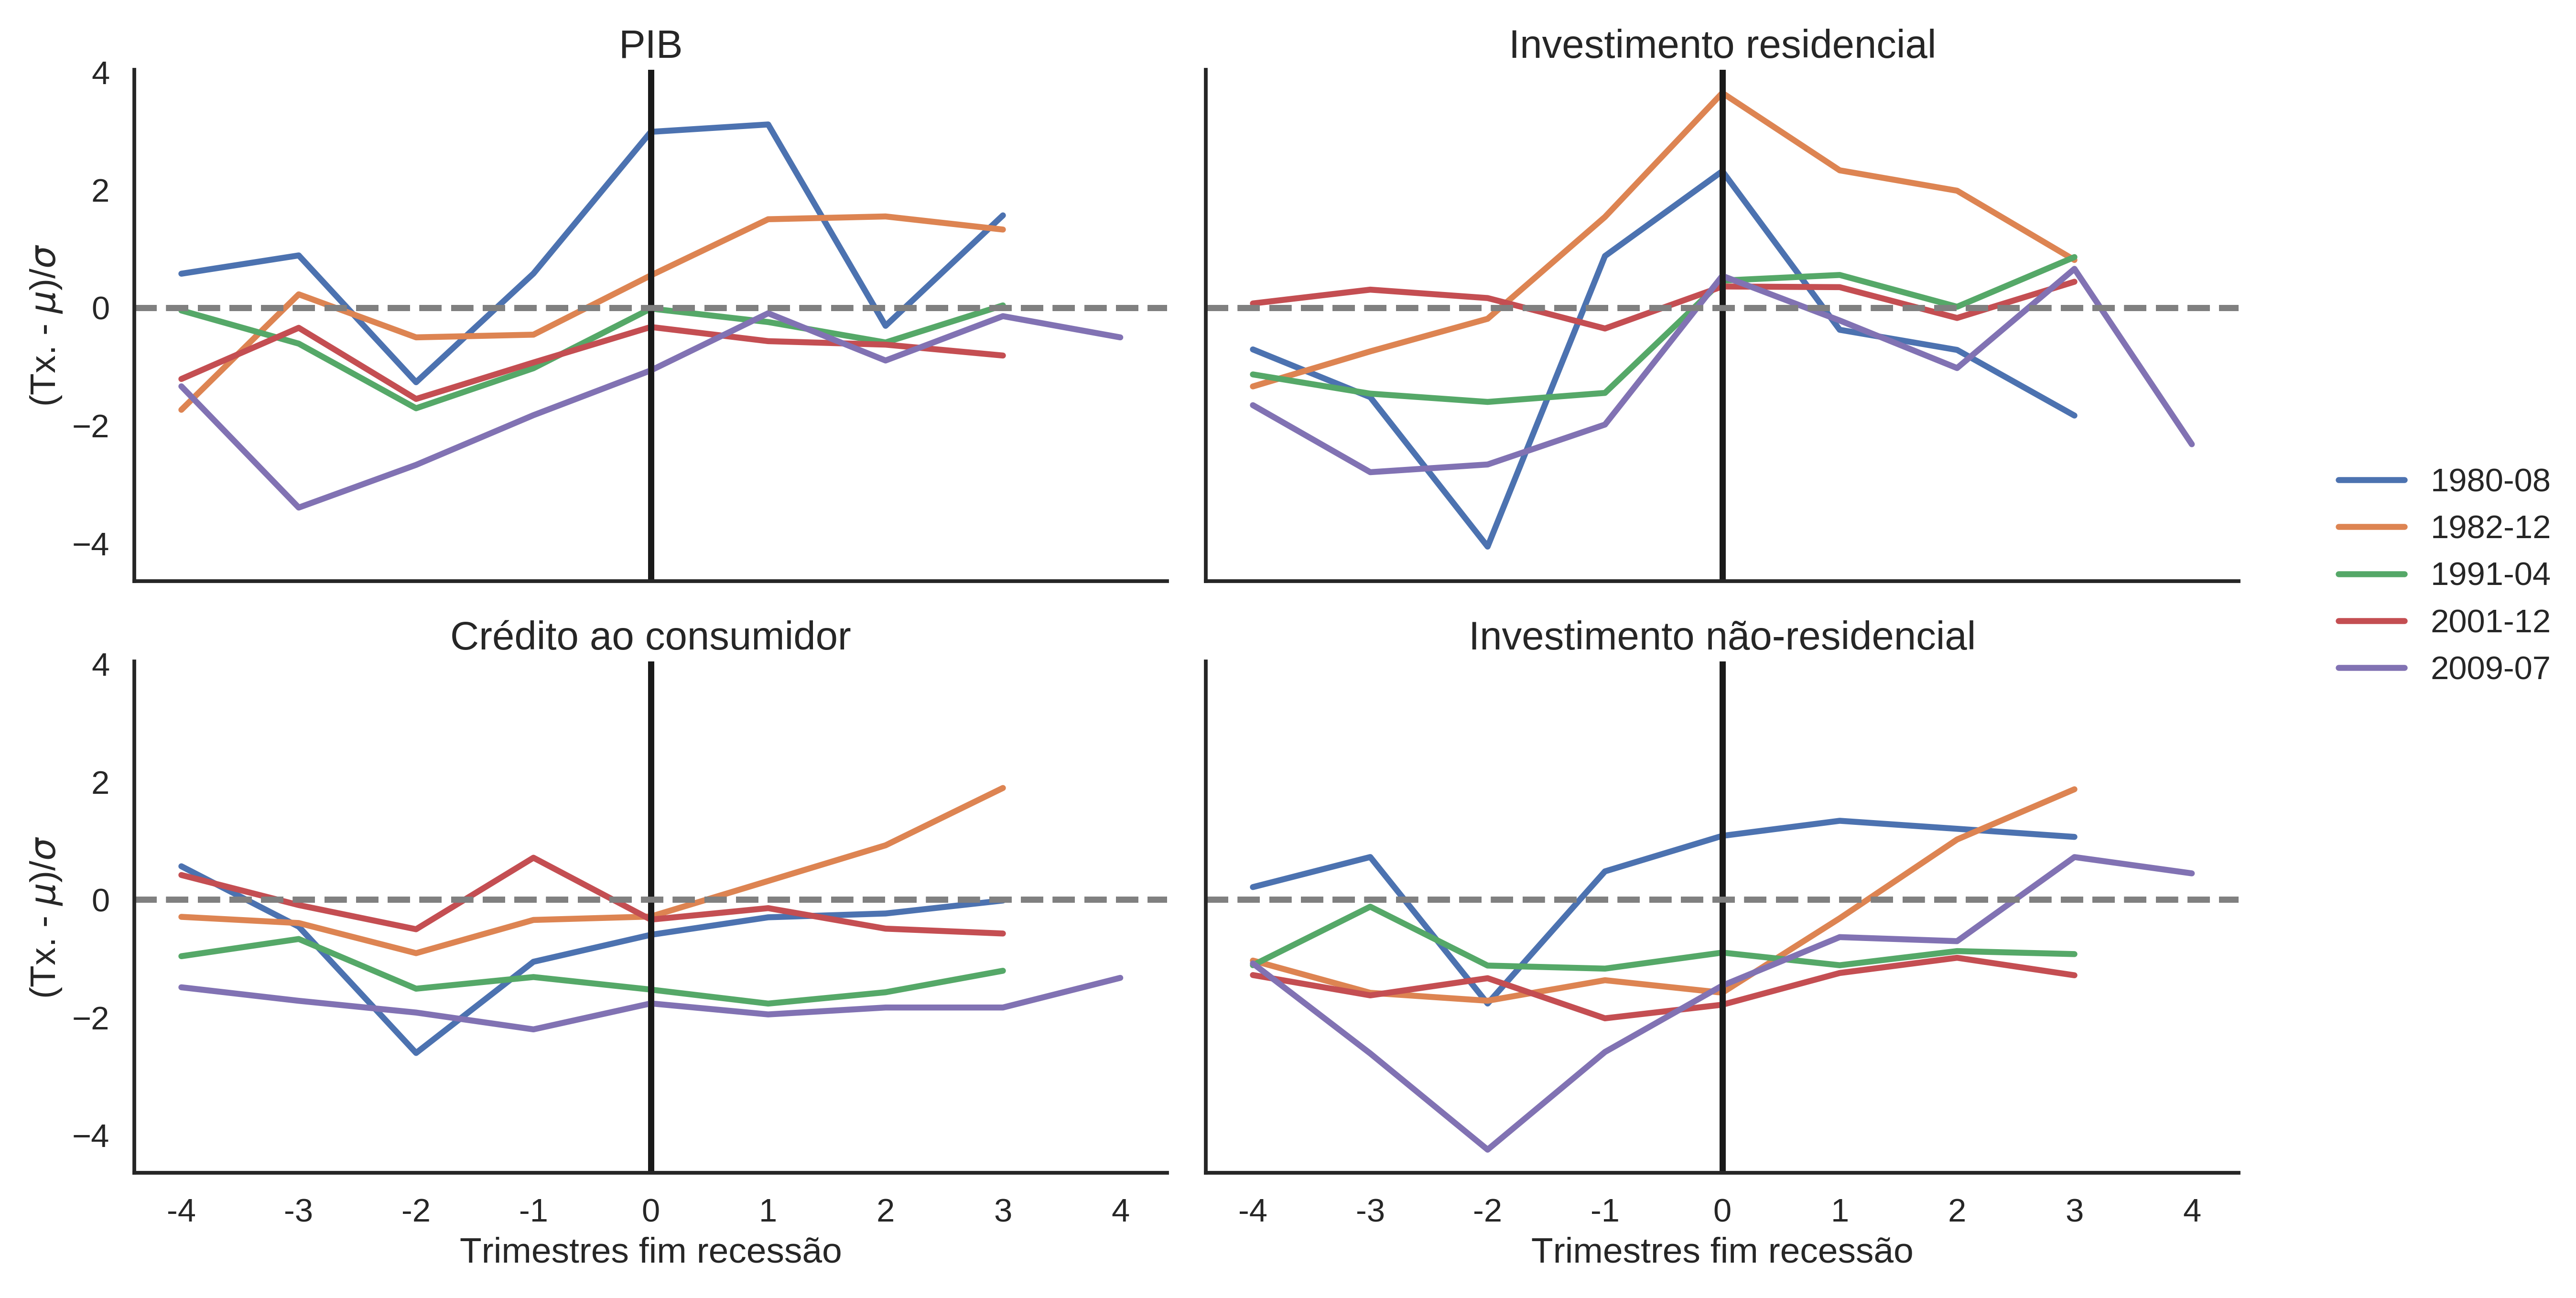
\includegraphics[width=\textwidth]{../../Dados/Fatos_Estilizados/figs/Centrado_Fim_Norm.png}
	\caption*{\textbf{Fonte:} Elaboração própria}
\end{figure}

%TODO Melhorar resolução do gráfico e linhas


Vale destacar que a importância do investimento residencial não se restringe ao longo prazo uma vez que exerce influência indireta na demanda agregada\footnote{
	A influência deste gasto, no entanto, não se restringe ao crescimento, mas se estende também para questões envolvendo desenvolvimento econômico como visto em um amplo debate iniciado por Duccio A. Turin \cite{pheng_revisit_1992}.}. 
De acordo com \textcite{teixeira_uma_2011}, imóveis são uma das formas de riqueza mais comuns entre as famílias norte-americanas, servindo de colateral para tomada de crédito\footnote{Como mostram \textcite{zezza_u.s._2008} e \textcite{barba_rising_2009} o consumo financiado por crédito foi um dos principais motores do crescimento da economia norte-americana no período que antecedeu a crise de 2008}. A forma de ``realizar'' o ganho de capital com a bolha imobiliária que ocorreu no período, sem precisar liquidar os imóveis, era justamente ampliando o endividamento à medida que o colateral (\textit{i.e.} imóveis) aumentava de valor \cite{teixeira_crescimento_2015}. 

DISTRIBUIÇÃO DE ATIVOS
%TODO Citar Survey

\begin{figure}[htb]
	\centering
	\caption{Distribuição de ativos por percentil de riqueza (1979=100)}
	\label{FigDistAtivos}
	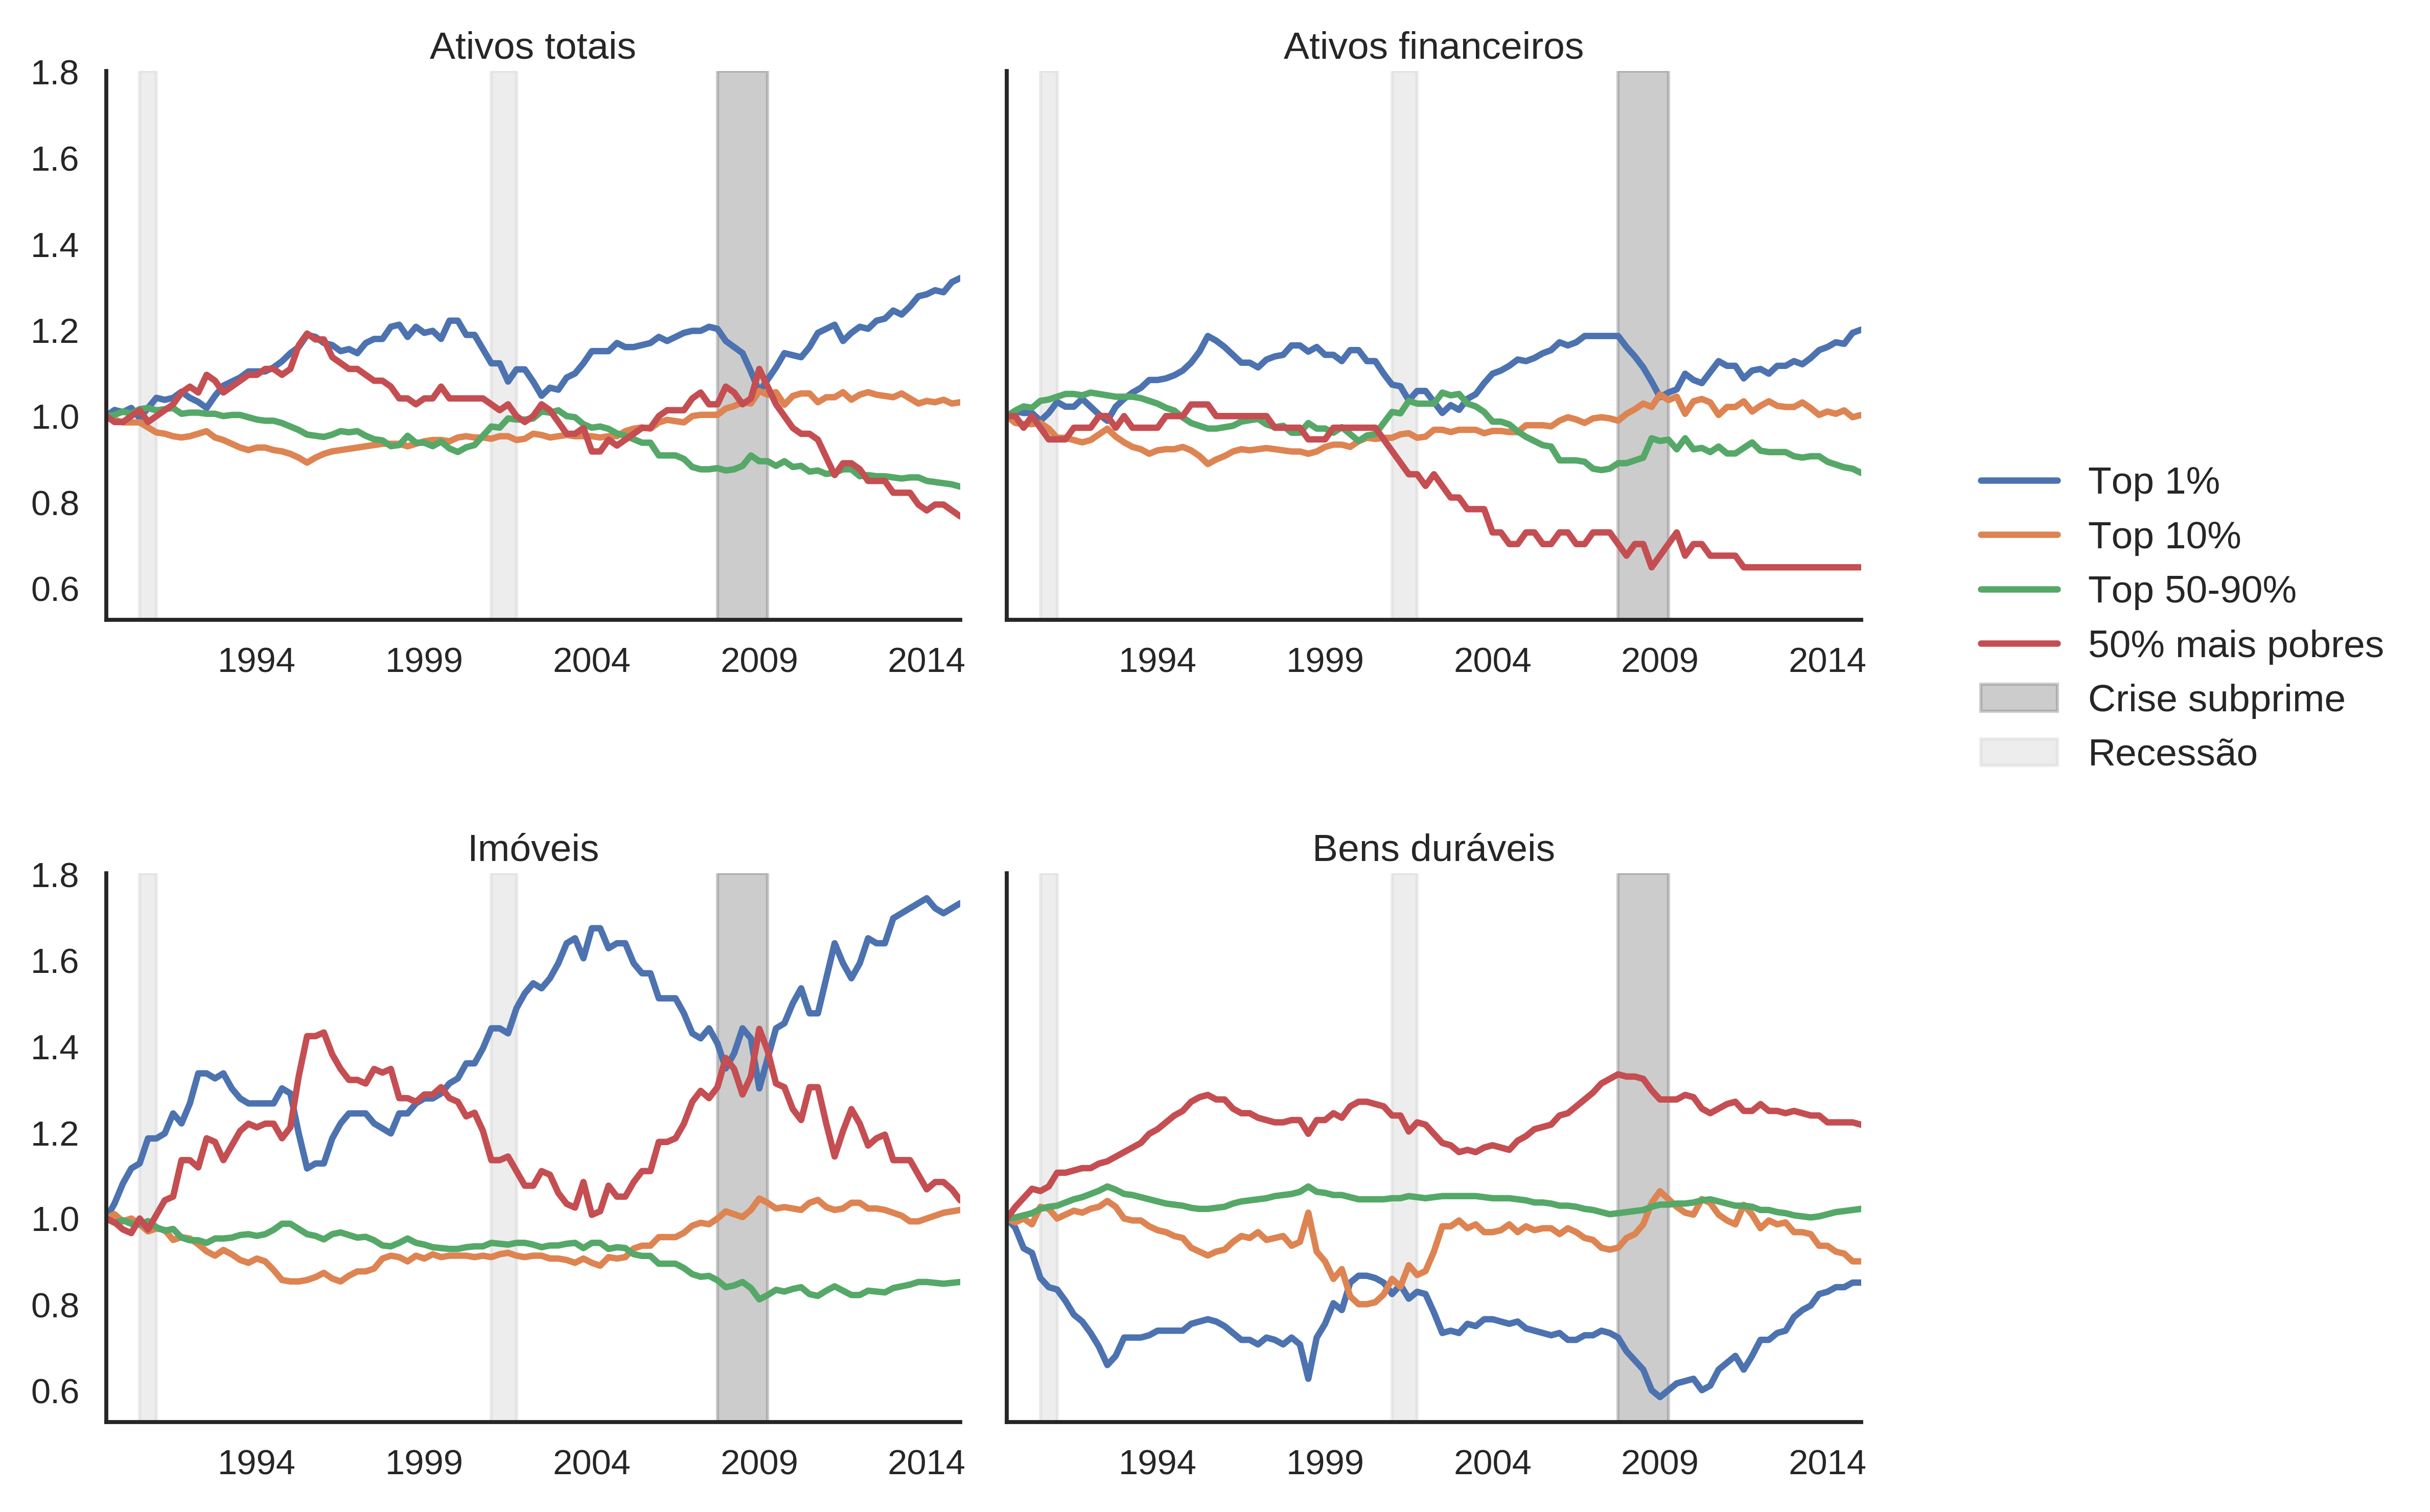
\includegraphics[width=\textwidth]{../../Dados/Fatos_Estilizados/figs/Distribuicao_Ativos.png}
	\caption*{\textbf{Fonte:} SURVEY, Elaboração própria}
\end{figure}


\begin{figure}[htb]
	\centering
	\caption{Distribuição de passivos por percentil de riqueza (1979=100)}
	\label{FigDistPassivos}
	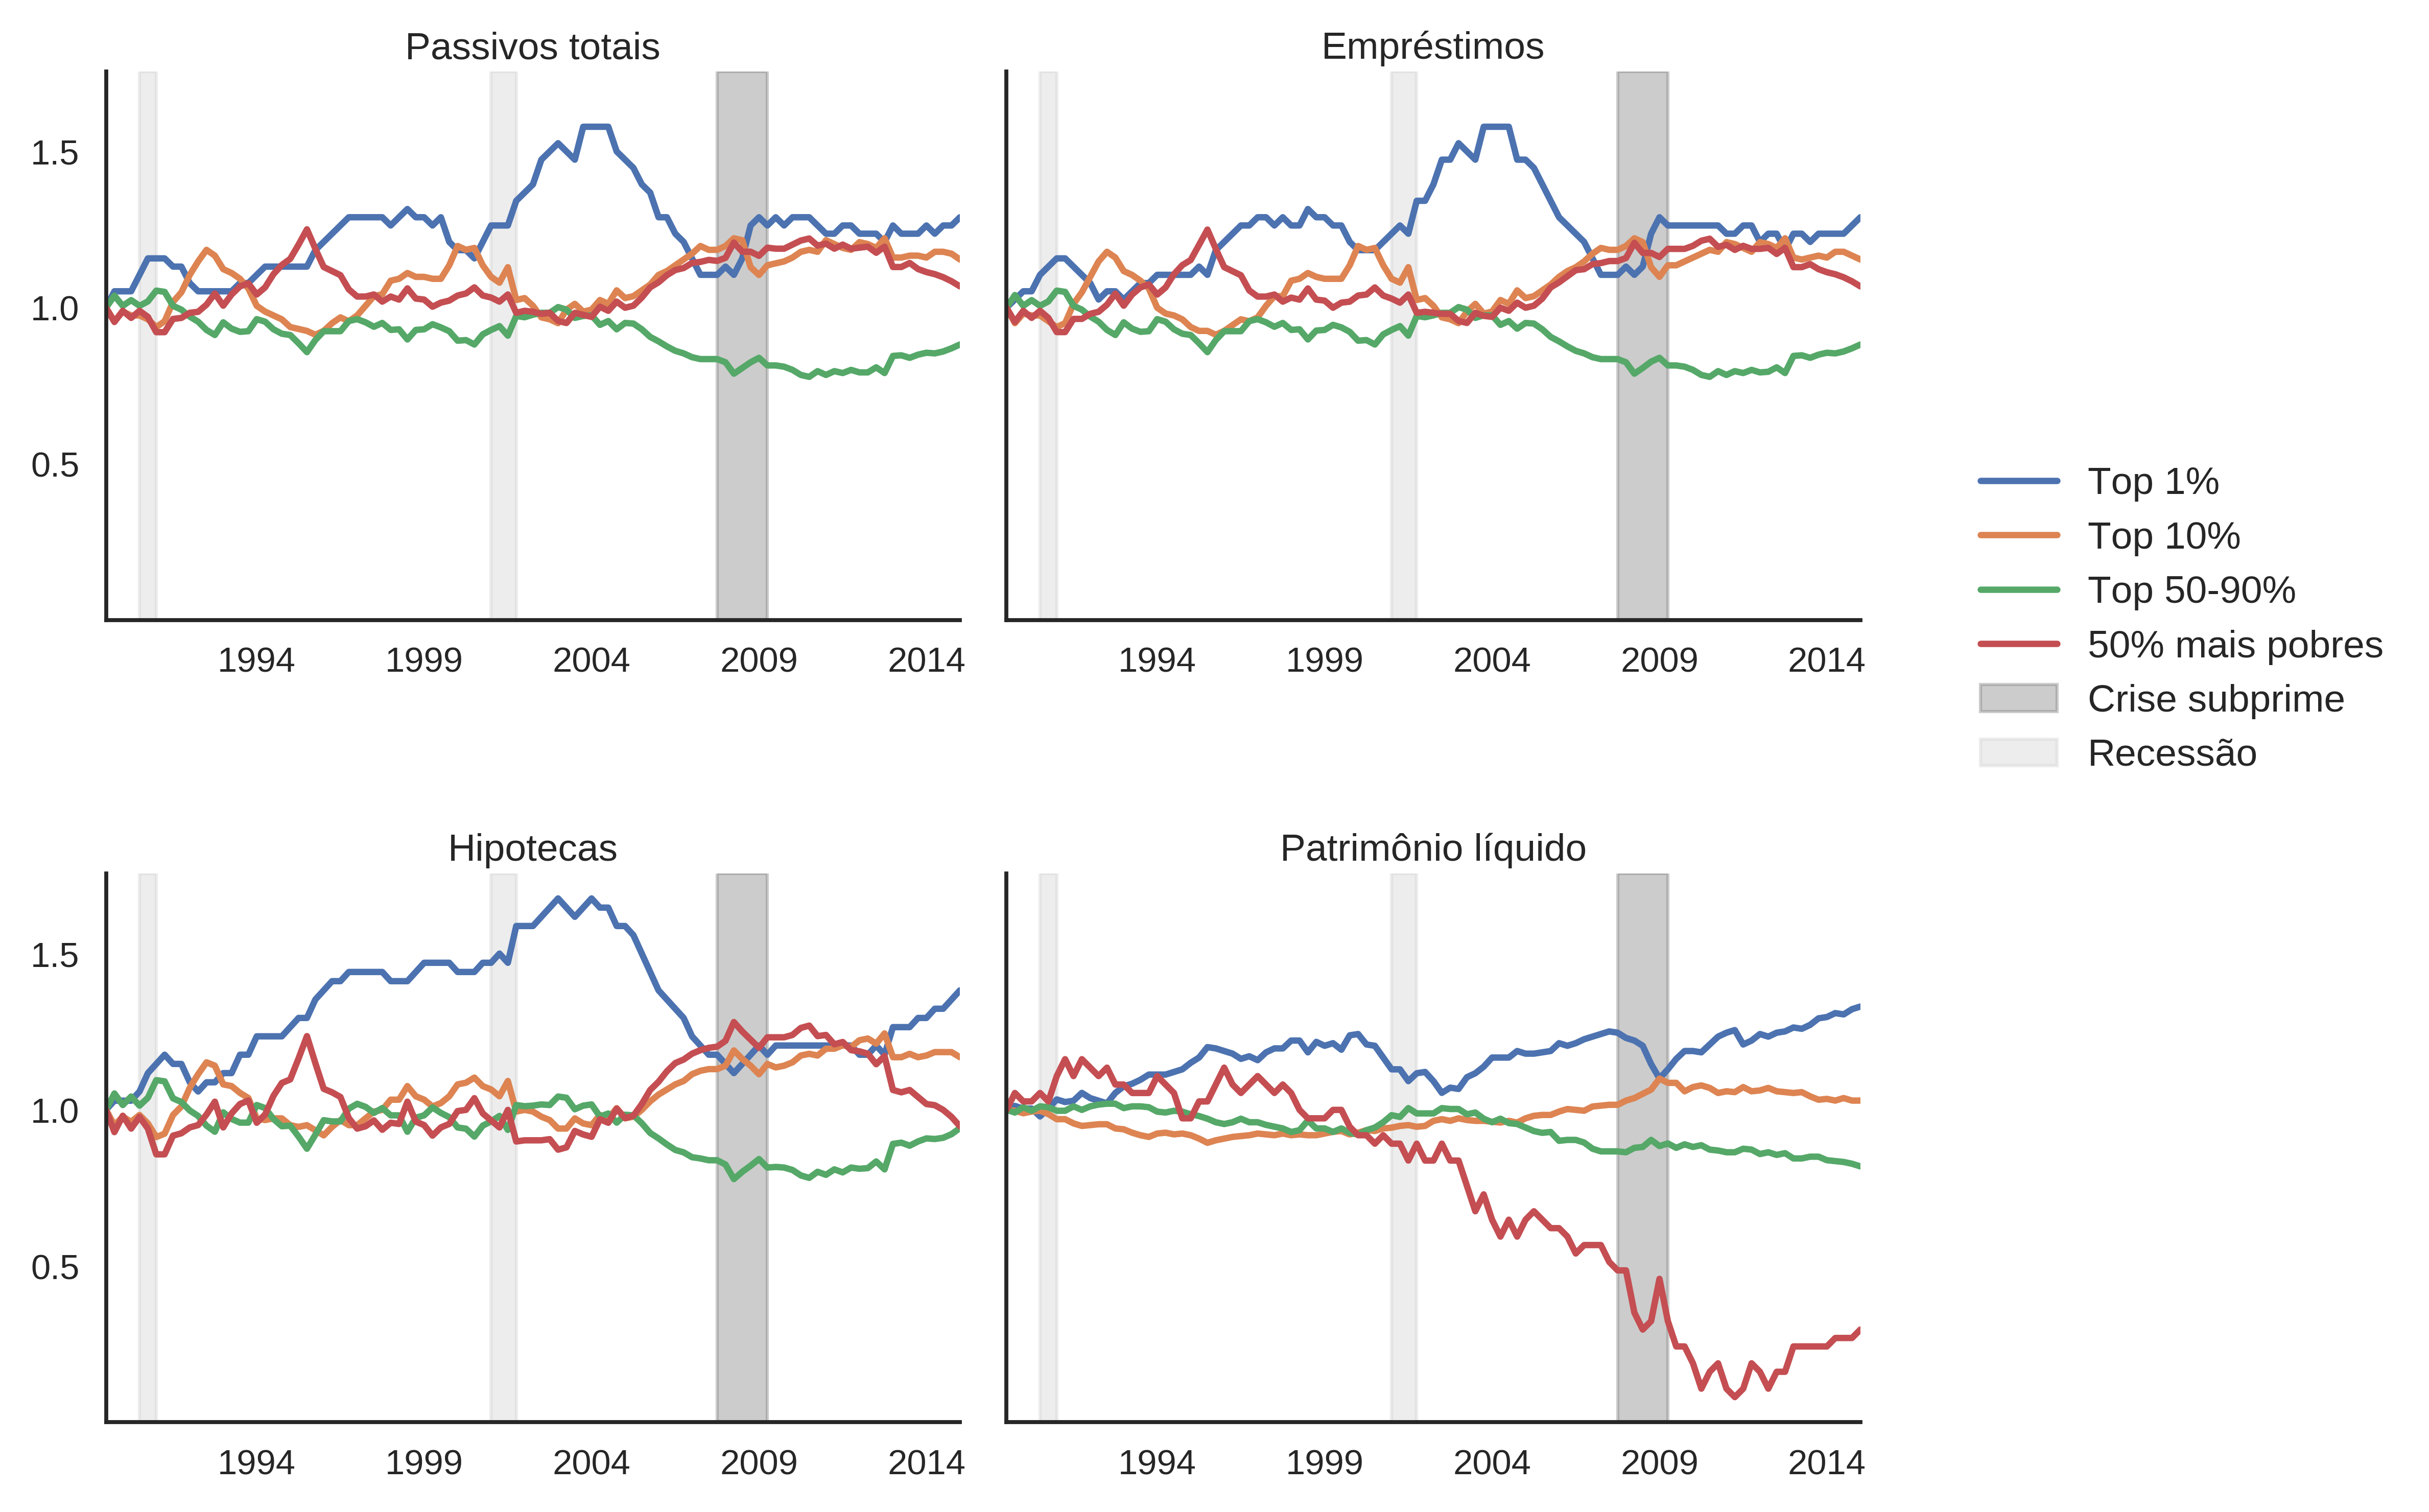
\includegraphics[width=\textwidth]{../../Dados/Fatos_Estilizados/figs/Distribuicao_Passivos.png}
	\caption*{\textbf{Fonte:} SURVEY, Elaboração própria}
\end{figure}


DISTRIBUIÇÃO DE PASSIVOS

DÍVIDA E PREÇO DOS IMÓVEIS

\begin{figure}[htb]
	\centering
	\caption{Dinâmica do endividamento das famílias e do preço dos imóveis (jan/2000=100)}
	\label{FigDividaPreco}
	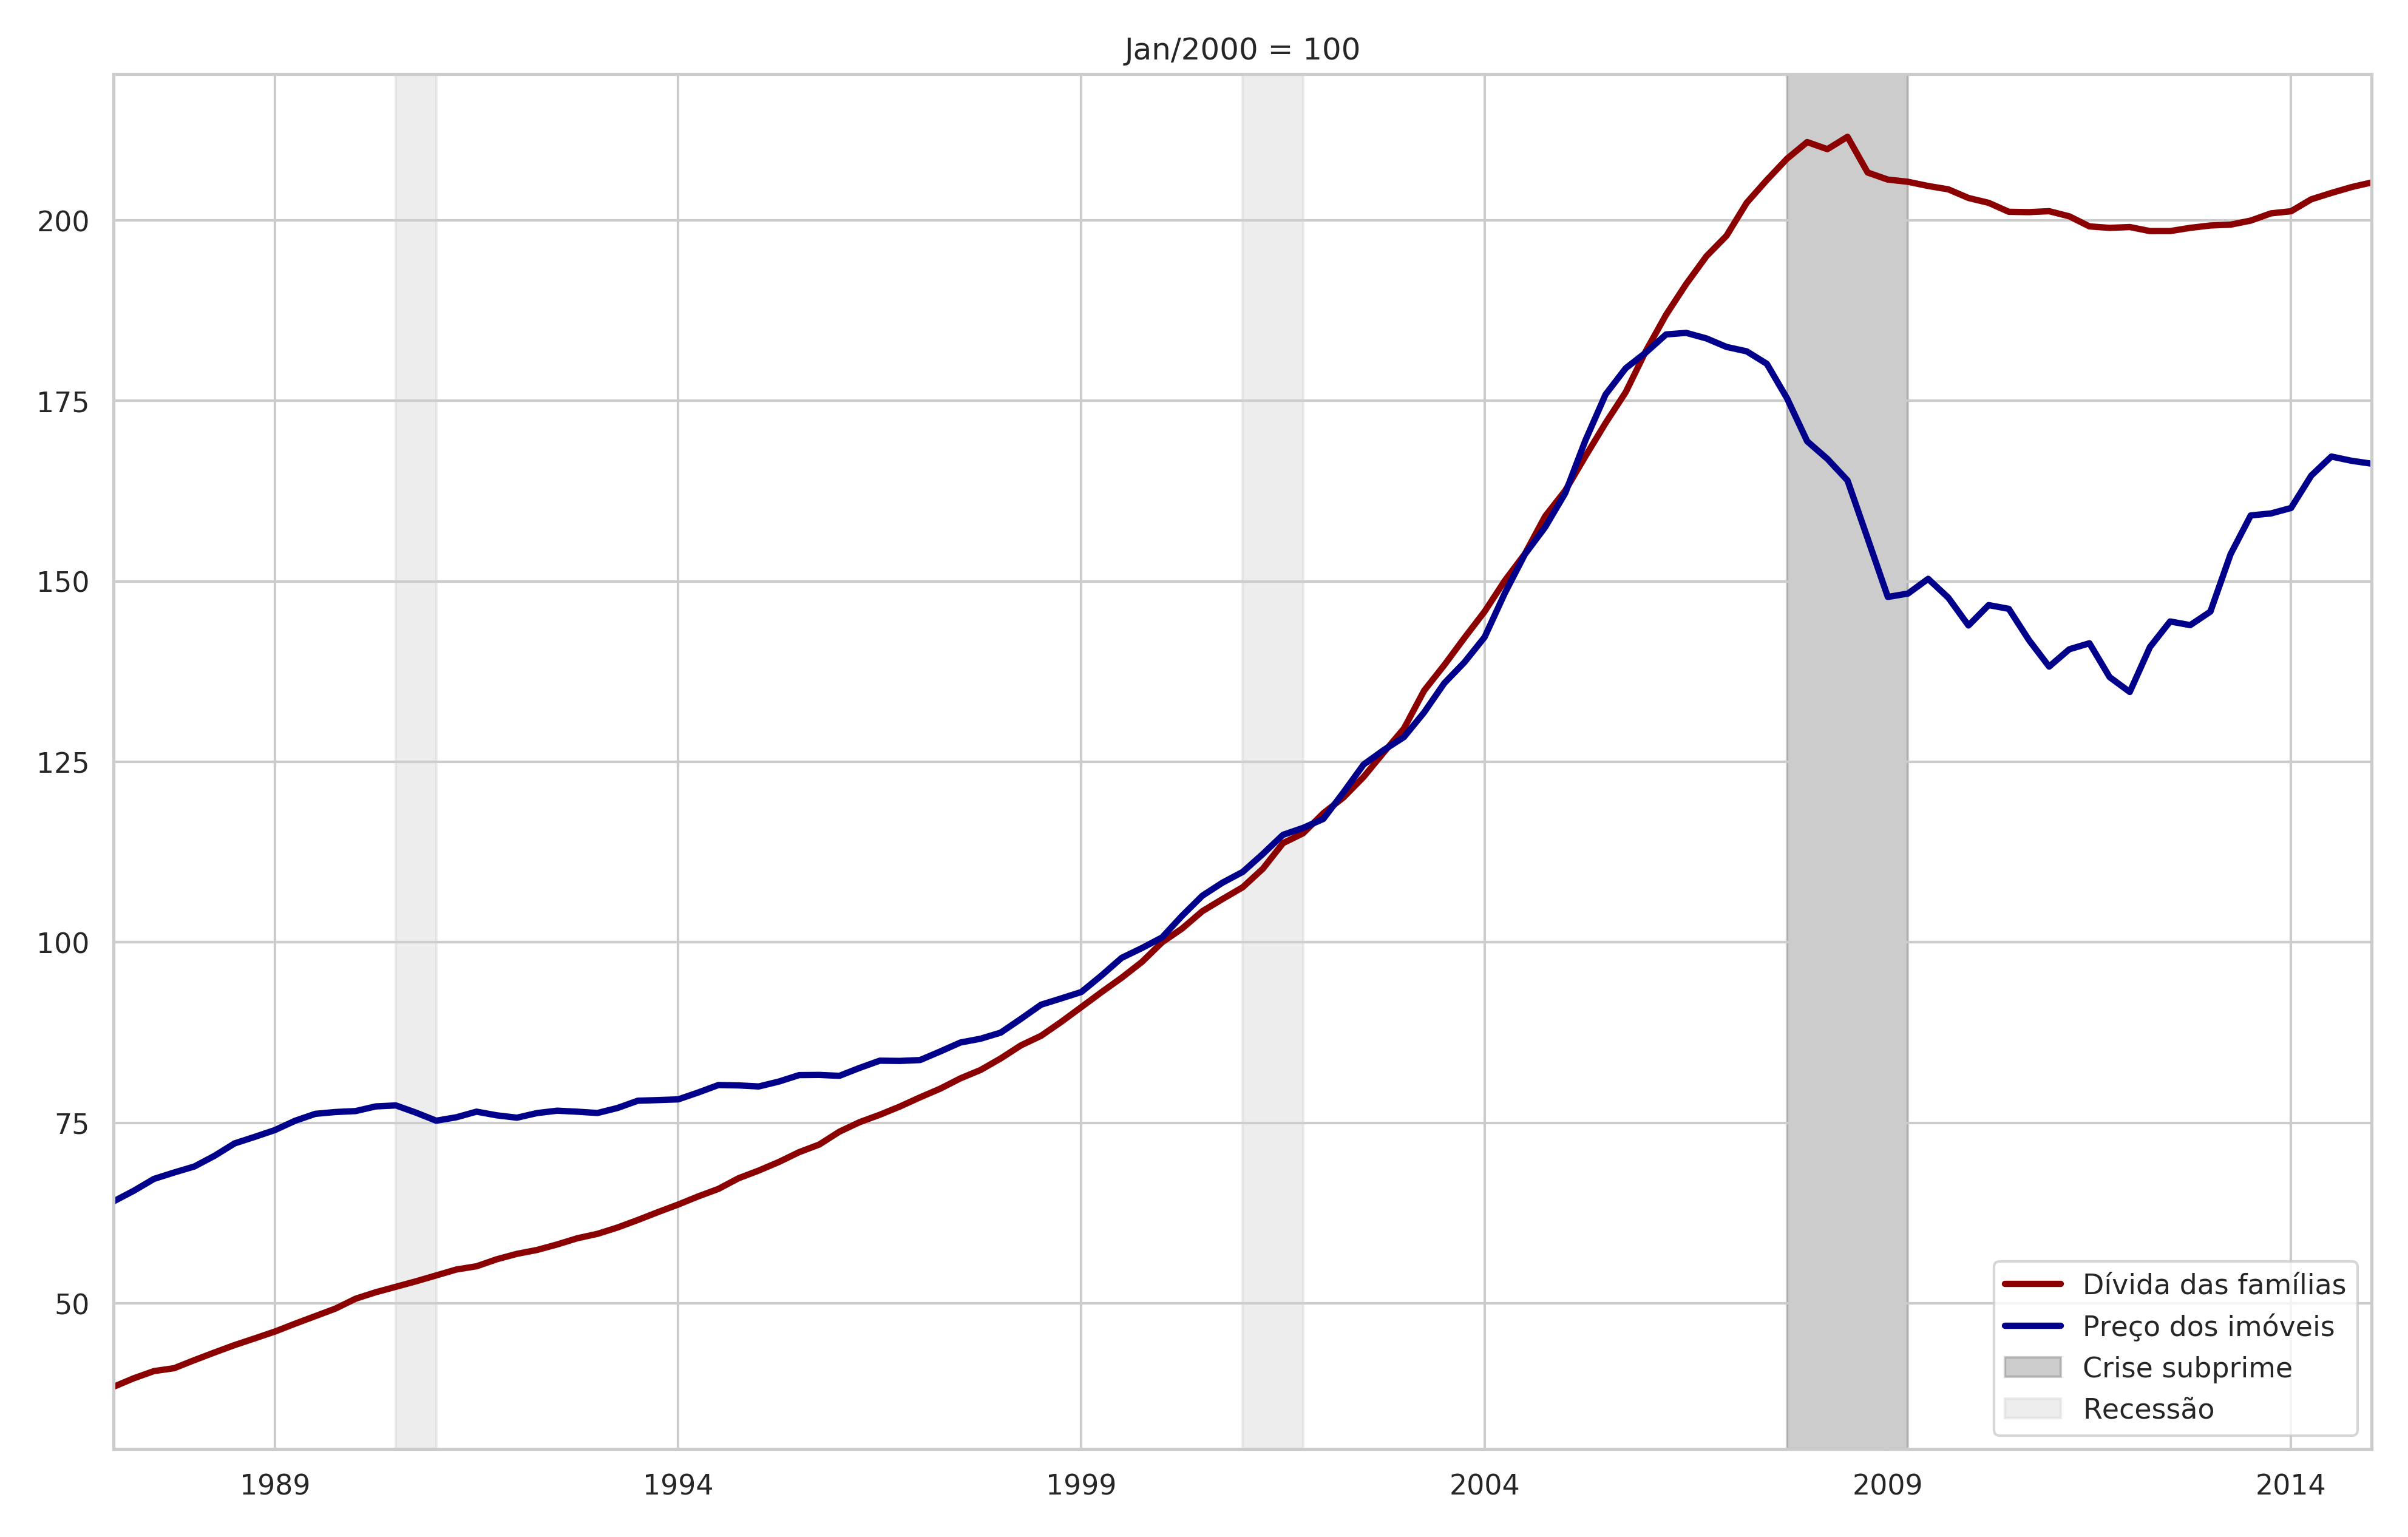
\includegraphics[width=\textwidth]{../../Dados/Fatos_Estilizados/figs/Divida_PrecoImoveis.png}
	\caption*{\textbf{Fonte:} U.S. Bureau of Economic Analisys, elaboração própria}
\end{figure}


POPULARIZAÇÃO DOS IMÓVEIS

\begin{figure}[htb]
	\centering
	\caption{Curva de concentração por tipos de imóveis}
	\label{FigConcentracao}
	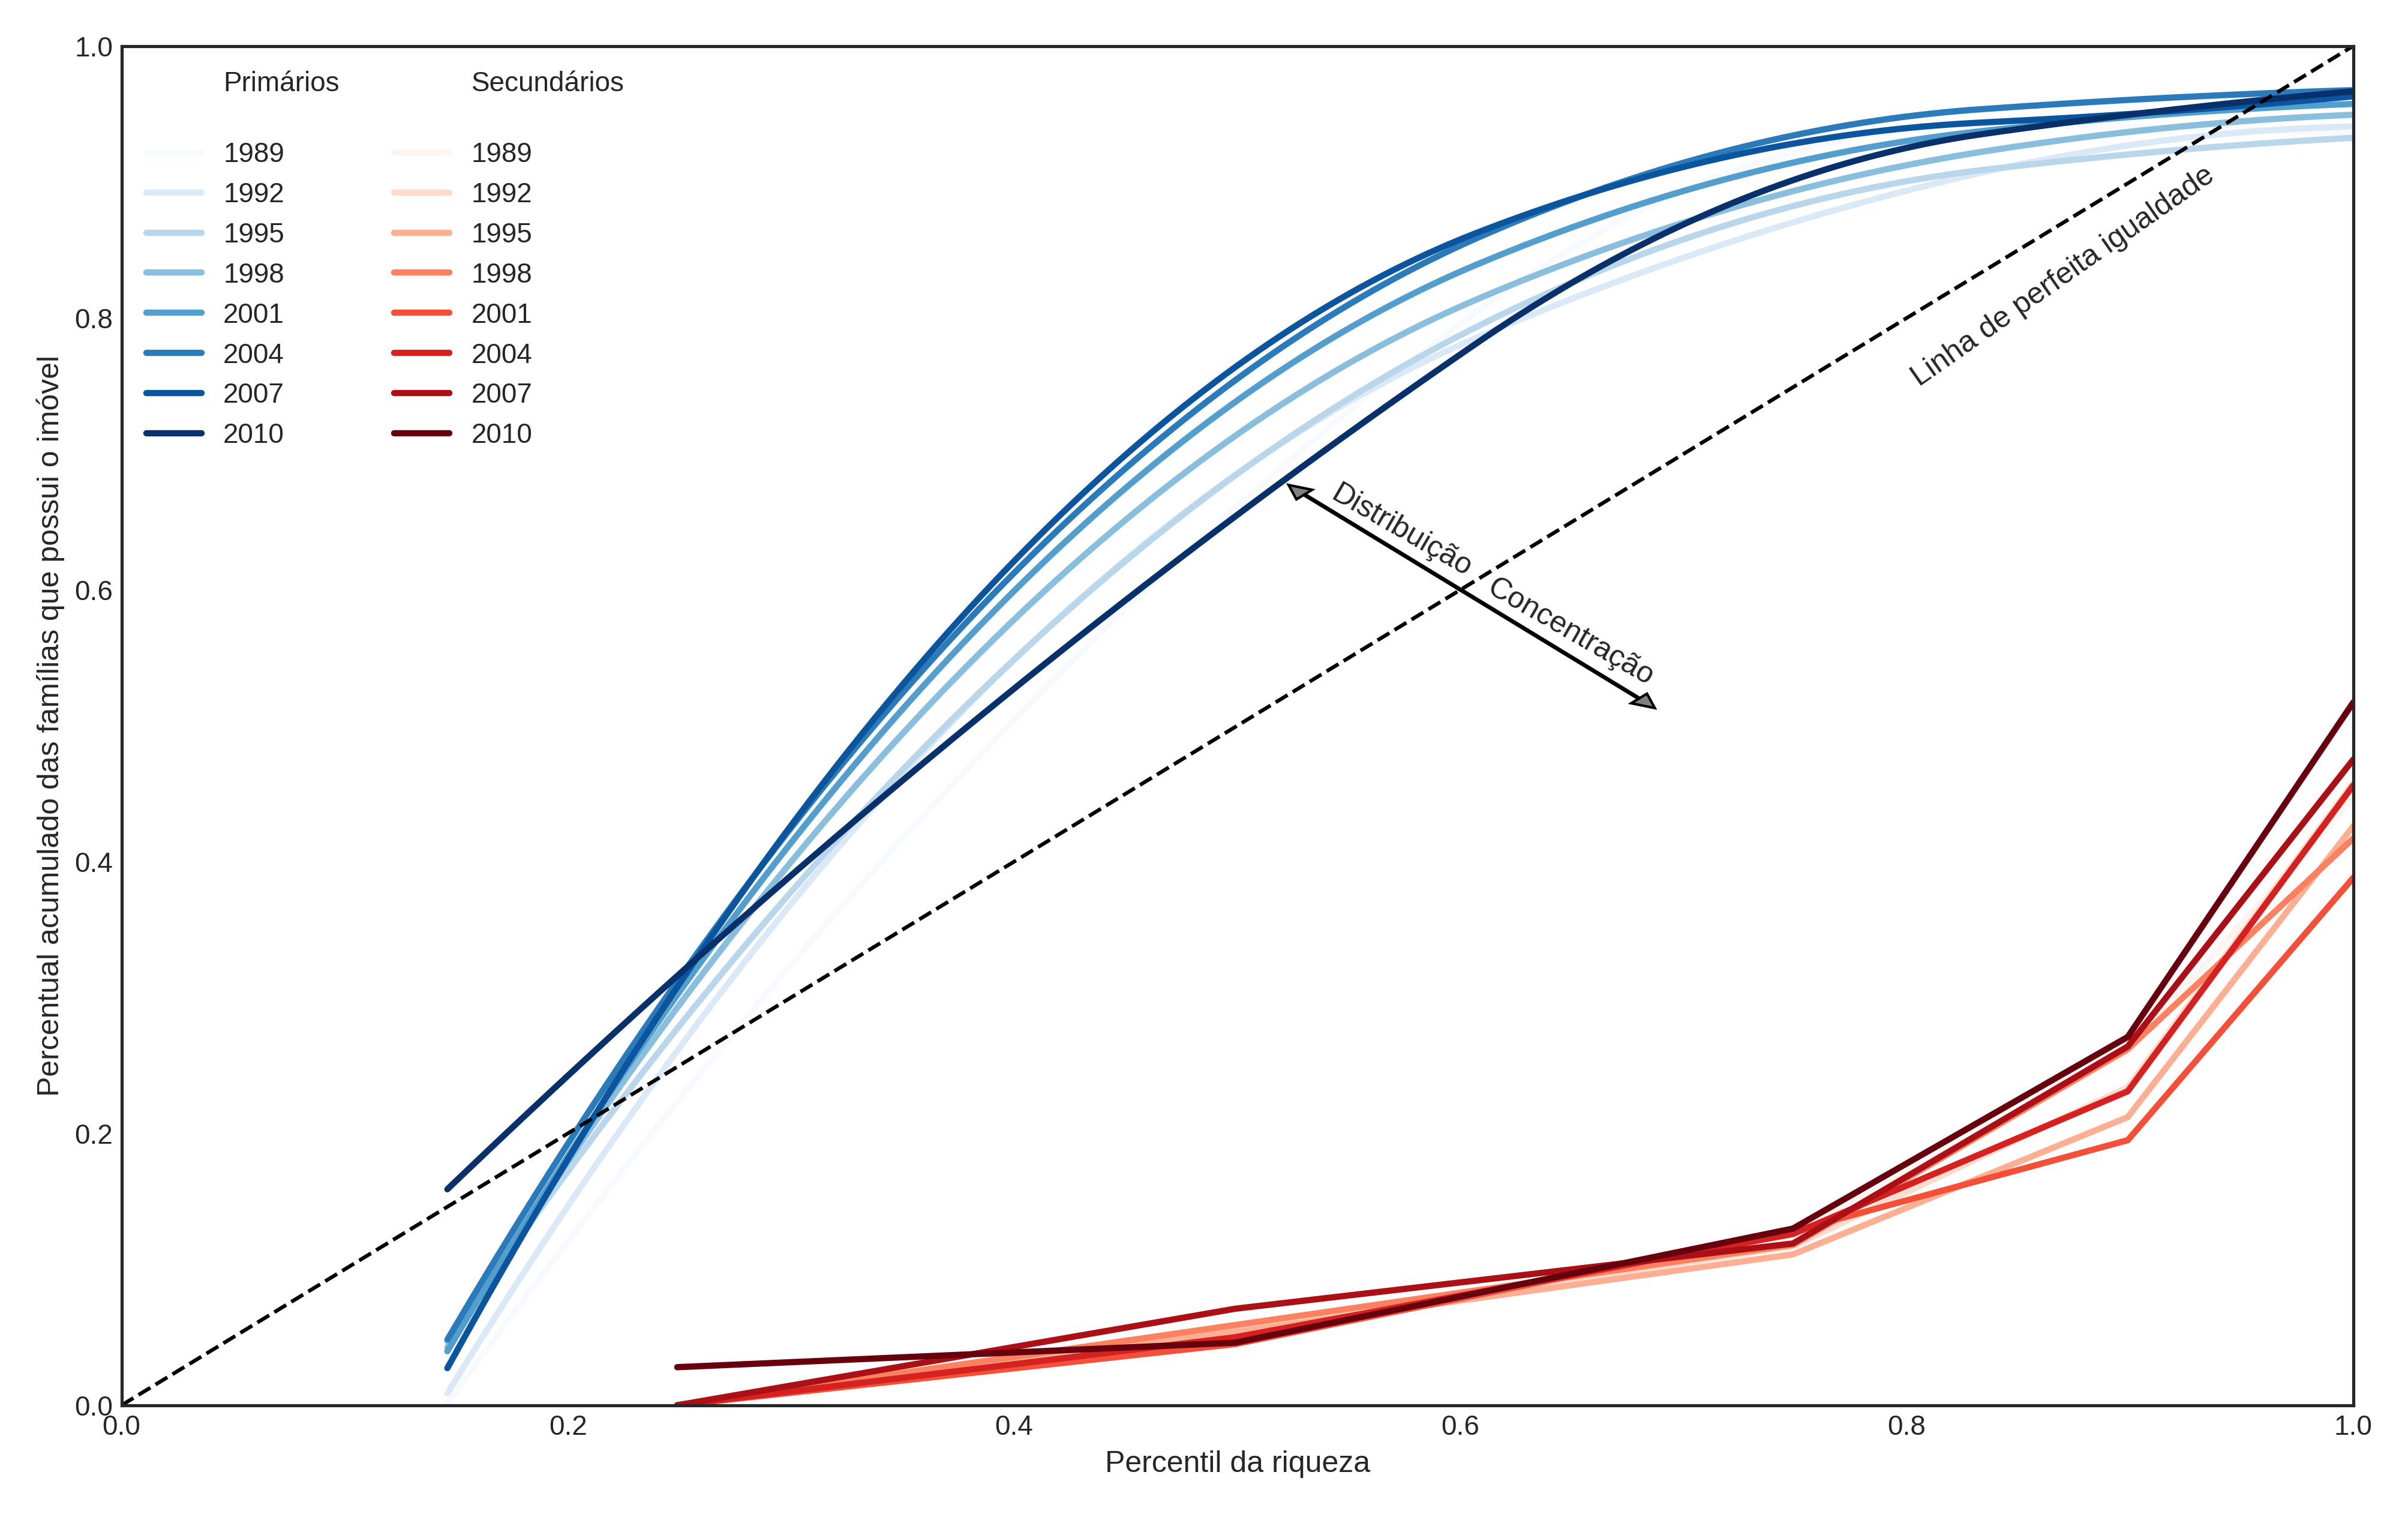
\includegraphics[width=\textwidth]{../../Dados/Fatos_Estilizados/figs/Concentracao_Imoveis.png}
	\caption*{\textbf{Fonte:} SURVEY, Elaboração própria}
\end{figure}

INFLAÇÃO DE IMÓVEIS?

TAXA PRÓPRIA E INVESTIMENTO RESIDENCIAL?





%Teixeira e a taxa própria
